Weight initialization plays a crucial role in model training. Even on the simplest model wrongly initialized weights (for example all constant or too large or too small) can lead to very slow convergence or prevent the model from converging at all (\cite{Kumar_2017}).

Xavier initialization, which is usually a default choice in many neural networks, works well for the most part for fully connected layers with tanh as activation function. There is also a study providing some insights into why Xavier initialization may not be the optimal choice for ReLU activations (\cite{Kumar_2017}). In the following samples \textit{fan\_in} denotes the maximum number of input signal units to a given layer and \textit{fan\_out} is the maximum number of output signal units from it. A definition of Xavier initialization can be found below:

Research of \cite{He_2015} also notices the problems with Xavier initialization for ReLU activations. The authors suggest a new robust method called He initialization that enables training of even extremely deep or wide network architectures with ReLU activations. This method was suggested by the \cite{Lachance_2020} paper and has been used in this reseach as well. He initialization draws samples from a truncated normal distribution:
\begin{equation}
	N(0, \sqrt{\frac{2}{\text{fan\_in}}})
\end{equation}

Default weight initialization of Conv2D layers in Python claims to use the initialization method of \cite{He_2015}, by calling it Kaiming uniform initialization, however after careful study of the PyTorch source code one realizes rather fast that the initialization approach used has nothing to do with the He initialization at all. Even the samples are drawn from the uniform distribution, although the paper clearly states that a normal distribution should be used. The definition of Kaiming uniform is provided below:
		\begin{align}
			std &= \sqrt{\frac{2}{fan\_in}} \\
			bou&nd = \sqrt{3 * std} \\
			Un&iform(-bound, bound)
		\end{align}

However, the naming is quite confusing and therefore two experiments have been conducted: first, the model predicting nuclei target was trained with the default weight initialization provided by PyTorch and then the initialization was switched to a true He initialization.

\begin{figure}[H]
	\begin{center}
		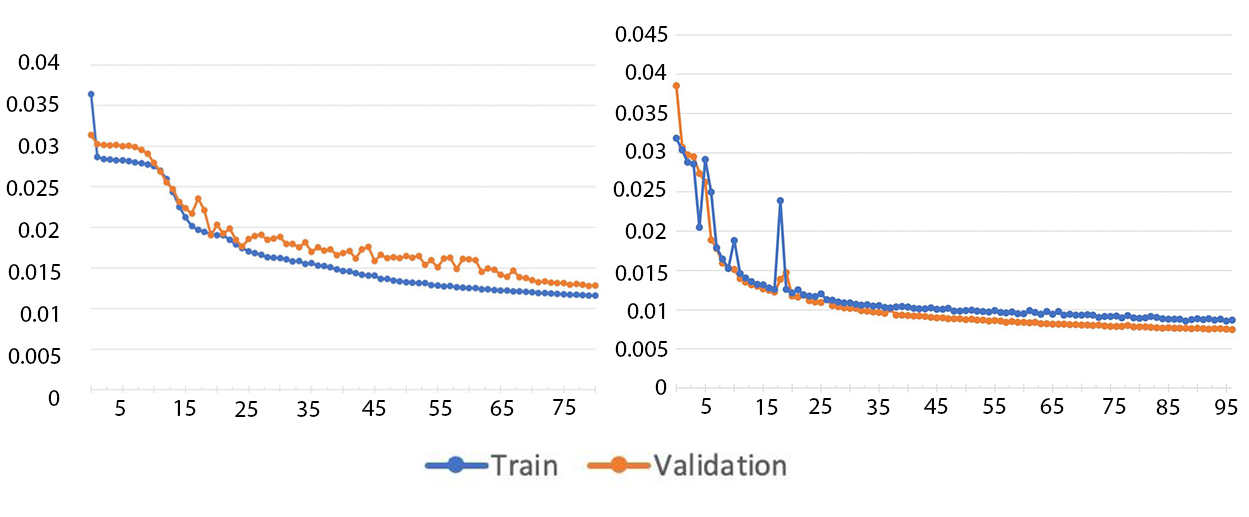
\includegraphics[width=0.8\linewidth]{bilder/nuclei/wi-no-wi.png}
		\caption{Nuclei training without (left) and with (right) custom weight initialization}\label{fig:wi}
	\end{center}
\end{figure}

The results of the experiments are presented in Figure \ref{fig:wi}. As can be seen, the loss in the left plots stagnates during the first few epochs and then begins to converge later. This is a symptom of a wrong initialization of the weights. Even after the convergence begins, the model still has a higher loss than the one on the right (around 0.012 in comparison to 0.007). However, the model on the right is not completely perfect as the loss still does not converge at the same speed everywhere. Although this might be not related to the weight initialization but more the to instability of the training in general as there were only few images used for these experiments.
